\documentclass[11pt]{article}
\usepackage[margin=0.95in]{geometry}
\usepackage{amsmath,amssymb}
\usepackage{graphicx}
\usepackage{booktabs,longtable,array}
\usepackage{xcolor}
\usepackage[hidelinks]{hyperref}
\usepackage{enumitem}
\usepackage{caption}
\setlist{itemsep=2pt,topsep=4pt}
\captionsetup{font=small,labelfont=bf}
\setlength{\parskip}{5pt}
\setlength{\parindent}{0pt}
\renewcommand{\arraystretch}{1.15}
\title{Recursion Under Delay: Phase 5 Report}
\author{}
\date{trm-delay-robust-scaling $\cdot$ Phase 5 report $\cdot$ 2026-10-10\\[2pt]One pre-registered stage, T2: does TD3's actor learning rate explain TRM's failure to train in Phase 4's Stage T? Stage note \texttt{stage\_T2.md} and figures (\texttt{figures/}) sit alongside; analysis in \texttt{.\allowbreak{}.\allowbreak{}/\allowbreak{}.\allowbreak{}.\allowbreak{}/\allowbreak{}experiments/\allowbreak{}analysis\_\allowbreak{}p5\_\allowbreak{}t2.\allowbreak{}json}.}
\begin{document}
\maketitle
\tableofcontents
\clearpage



\section*{Executive summary}\addcontentsline{toc}{section}{Executive summary}



\textbf{Why Phase 5.} Phase 4's Stage T reran Phase 3's capacity contrast (G1) under TD3 with \texttt{td3.yaml} unchanged. Its gate GT passed on sign, but with a recorded caveat: TRM 788k did not train (2/12 runs learned; its critic loss rose through training) while every MLP run learned, so the pass reflected an optimisation failure, not a deficit of Phase 3's kind. The caveat named the likely cause, untested: \texttt{td3.yaml}'s actor learning rate, 1e-3, is ten times the DDPG rate (1e-4) at which TRM had trained normally. Phase 5 tests that one explanation.



\textbf{What was run.} A pre-registered stage (plan frozen 2026-10-10; rule GT2 and amendment P5-1 in \texttt{experiments/\allowbreak{}phase5/\allowbreak{}gates.\allowbreak{}json}), 36 Katana GPU jobs from a frozen snapshot with code byte-identical to Stage T's. Pendulum-v1, TD3 with only \texttt{arch.actor\_lr} overridden, conditions C0 and C1, seeds 1--6, 200 episodes. TRM 788k at actor LR 1e-4 and 3e-4; its 1e-3 arm is Stage T's 12 runs (P5-1); control MLP 788k at 1e-4.



\textbf{What it found.}



\begin{center}\small\begin{tabular}{>{\raggedright\arraybackslash}p{0.214\linewidth}>{\raggedright\arraybackslash}p{0.095\linewidth}>{\raggedleft\arraybackslash}p{0.427\linewidth}>{\raggedleft\arraybackslash}p{0.142\linewidth}}
\toprule
Arm & Actor LR & Runs learned (final avg-100 > $-$1000) & Median final \\
\midrule
TRM 788k & 1e-4 & 12/12 & $-$187.69 \\
TRM 788k & 3e-4 & 11/12 & $-$234.56 \\
TRM 788k (Stage T) & 1e-3 & 2/12 & $-$1389.27 \\
MLP 788k & 1e-4 & 12/12 & $-$176.14 \\
MLP 788k (Stage T) & 1e-3 & 12/12 & $-$175.92 \\
\bottomrule
\end{tabular}\end{center}



\emph{Source: \texttt{experiments/\allowbreak{}analysis\_\allowbreak{}p5\_\allowbreak{}t2.\allowbreak{}json} (\texttt{arms}).}



\textbf{GT2: "LR explains"} (as recorded in \texttt{gates.json}). At the LR-matched setting (both at 1e-4), TRM 788k $-$ MLP 788k is a median $-$12.98, with 2/12 pairs positive (two-sided p = 0.039). With unequal LRs (TRM 3e-4, MLP 1e-4) it is $-$53.6, 0/12.



\textbf{What it changes.} Stage T's failure was an actor-learning-rate effect. At a DDPG-like actor rate TRM trains under TD3, and the capacity contrast shows the same direction and sign count as Phase 3's G1 under DDPG ($-$27.1, 2/12), with a smaller median: a modest, consistent deficit with a worse value fit (late critic loss 1.50$\times$ the MLP's, 12/12). The caveat on GT is resolved, and Phase 3's architectural attribution now holds under two algorithms at matched, sensible learning rates. A new, exploratory observation: TRM is far more sensitive to the actor learning rate than the MLP, which is unaffected by a tenfold change. \textbf{The practical recommendation is unchanged: use the MLP.}



\begin{figure}[htbp]\centering
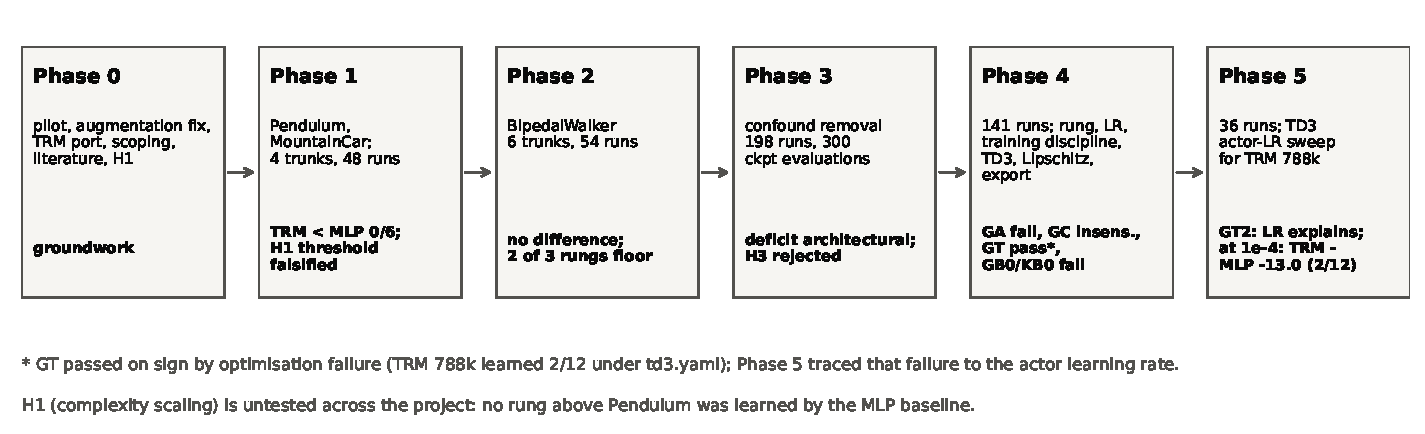
\includegraphics[width=\linewidth,height=0.42\textheight,keepaspectratio]{figures/p5_f3_project_map.pdf}
\caption{The project's phases, with Phase 5 added}
\end{figure}



\medskip



\section*{1. Why Phase 5}\addcontentsline{toc}{section}{1. Why Phase 5}



Every contrast in Phases 1--3 used DDPG. Phase 4 added Stage T (amendment T-1) to test whether Phase 3's central attribution, G1, held under a second algorithm. G1 had found that TRM trails a parameter-matched MLP at both 135k ($-$50.2, 0/12) and 788k ($-$27.1, 2/12), while a 5.8$\times$ larger MLP changes nothing ($-$3.8, 5/12). Stage T used \texttt{td3.yaml} unchanged and no tuning for any trunk.



The result was ambiguous in a specific way. Both MLPs reproduced their DDPG medians in every run, but TRM 788k stayed near random policy in 10 of 12 runs, with its critic loss rising from 118.6 (episodes 51--75) to 560.9 (last quarter). GT's sign rule cannot tell a deficit from a failure to train, so the pass said nothing about the size of an architectural deficit under TD3. The author also cited this as one of the two reasons for not running the TD3 complexity stage B1 (Phase 4 amendment K-3).



Phase 4's evidence pointed to one setting. \texttt{td3.yaml} sets the actor learning rate to 1e-3, against the 1e-4 of the project's DDPG configuration (the rate Lillicrap et al., 2016, used), and Phase 4's Stage C had shown under DDPG that tripling TRM's actor rate already hurts it (all three 3e-4 cells below the default in 3/3 seeds). The other TD3 differences (batch 256, twin critics, target-policy smoothing, policy delay 2, 10,000-step warmup) applied equally to the MLPs, which were unaffected. Phase 5 is the smallest experiment that tests the actor-rate explanation: lower that one setting and see whether TRM trains.



The framing is unchanged from Phase 4: the thesis assesses whether TRM's architecture, ported as faithfully as the setting allows, works as a model-free RL trunk. Phase 5 does not redesign or tune the architecture; it removes one confound from one comparison.



\section*{2. What was pre-registered}\addcontentsline{toc}{section}{2. What was pre-registered}



The plan (\texttt{phase5/\allowbreak{}plan/\allowbreak{}plan.\allowbreak{}md}) was frozen on 2026-10-10, before any Phase 5 data, with its rule machine-readable in \texttt{experiments/\allowbreak{}phase5/\allowbreak{}gates.\allowbreak{}json}. \texttt{experiments/\allowbreak{}phase5/\allowbreak{}gates\_\allowbreak{}eval.\allowbreak{}py} evaluates it and writes the outcome only when all arms are complete; it never edits a rule or frozen value.



\begin{center}\small\begin{tabular}{>{\raggedright\arraybackslash}p{0.119\linewidth}>{\raggedright\arraybackslash}p{0.815\linewidth}}
\toprule
Item & Pre-registered value \\
\midrule
Setting & Pendulum-v1, TD3 (\texttt{td3.yaml}), only \texttt{arch.actor\_lr} overridden; 200 episodes; C0 and C1; seeds 1--6 \\
Actor LRs & 1e-4, 3e-4, 1e-3 for TRM 788k; 1e-4 for the MLP 788k control; critic LR 1e-3 throughout \\
"Learned" & final avg-100 > $-$1000 \\
GT2 & "LR explains the TD3 failure" if TRM 788k learns in $\geq$ 10/12 runs at some actor LR < 1e-3; then TRM 788k $-$ MLP 788k (actor LR 1e-4) at that LR, n = 12 (seed, condition) pairs, sign test, two-sided p. If both 1e-4 and 3e-4 pass, both contrasts are reported; 1e-4 is LR-matched and primary, 3e-4 compares unequal actor LRs \\
Secondary & late critic-loss medians (last quarter), eval last-5, MLP learned count against Stage T's MLP 788k at 1e-3 \\
Amendment P5-1 (before data) & TRM 788k at 1e-3 reuses Stage T's 12 runs (same configuration, byte-identical code); 36 new jobs \\
\bottomrule
\end{tabular}\end{center}



\emph{Source: \texttt{experiments/\allowbreak{}phase5/\allowbreak{}gates.\allowbreak{}json} (\texttt{frozen\_values}, \texttt{gates[GT2].\allowbreak{}rule}, \texttt{amendments}); \texttt{phase5/\allowbreak{}plan/\allowbreak{}plan.\allowbreak{}md} \S{}2, \S{}5.}



The plan also recorded four threats before data (\S{}7 below): the coarseness of the threshold, the three-point grid, the MLP control at one LR, and cross-GPU reproducibility of reused runs.



\section*{3. Methodology}\addcontentsline{toc}{section}{3. Methodology}



\subsection*{3.1 Environment, algorithm and conditions}\addcontentsline{toc}{subsection}{3.1 Environment, algorithm and conditions}



\begin{itemize}
\item \textbf{Pendulum-v1} (Gymnasium; Towers et al., 2024): 3-D observation, 1-D torque in [$-$2, 2], 200-step episodes, dense cost. The one environment every trunk learned in Phases 1--4 and the site of Stage T, so the result connects directly to it.
\item \textbf{TD3} (Fujimoto et al., 2018; \texttt{conf/\allowbreak{}arch/\allowbreak{}td3.\allowbreak{}yaml}): critic LR 1e-3, batch 256, 10,000 random-action warmup steps (50 of the 200 episodes), Gaussian exploration noise 0.1 of the action range, twin critics, policy delay 2, target-policy noise 0.2 clipped at 0.5, $\gamma$ = 0.99, $\tau$ = 0.005, buffer 200,000. Only the actor learning rate varies.
\item \textbf{Conditions:} C0, no delay; C1, fixed d = 1 with the one-slot queue in the observation and no previous-action input (Phase 3 Stage 1's and Stage T's conditions).
\end{itemize}



\subsection*{3.2 Trunks and parameter counts}\addcontentsline{toc}{subsection}{3.2 Trunks and parameter counts}



TRM 788k (\texttt{trm}), the project's port of TRM (Jolicoeur-Martineau, 2025): one SwiGLU/RMSNorm reasoning cell (two layers, expansion 4, hidden 128), \texttt{H\_cycles = 3}, \texttt{L\_cycles = 6}, one-step gradient truncation, latent reset every call; the port used throughout the project. MLP 788k (\texttt{dnn\_large}): \texttt{[624, 624]}, ReLU. Under TD3 the counts include twin critics (excluding targets): TRM 788k 1,181,443 at C0 and 1,181,827 at C1; MLP 788k 1,180,611 and 1,182,483 (\texttt{figures/\allowbreak{}derived\_\allowbreak{}numbers\_\allowbreak{}p5.\allowbreak{}json}). The labels name the DDPG-basis configurations.



\subsection*{3.3 Arms, seeds, budget}\addcontentsline{toc}{subsection}{3.3 Arms, seeds, budget}



\begin{center}\small\begin{tabular}{>{\raggedright\arraybackslash}p{0.118\linewidth}>{\raggedright\arraybackslash}p{0.118\linewidth}>{\raggedleft\arraybackslash}p{0.063\linewidth}>{\raggedright\arraybackslash}p{0.578\linewidth}}
\toprule
Arm & Actor LR & Runs & Source \\
\midrule
TRM 788k & 1e-4 & 12 & new (\texttt{phase5/\allowbreak{}results/\allowbreak{}results\_\allowbreak{}p5t2/\allowbreak{}}) \\
TRM 788k & 3e-4 & 12 & new \\
TRM 788k & 1e-3 & 12 & Stage T, reused (P5-1; \texttt{phase4/\allowbreak{}results/\allowbreak{}results\_\allowbreak{}p4t/\allowbreak{}}) \\
MLP 788k & 1e-4 & 12 & new \\
MLP 788k & 1e-3 & 12 & Stage T, for the secondary comparison only \\
\bottomrule
\end{tabular}\end{center}



Each arm is 6 seeds $\times$ 2 conditions. 36 new training runs.



\subsection*{3.4 Metrics and statistics}\addcontentsline{toc}{subsection}{3.4 Metrics and statistics}



\begin{itemize}
\item \textbf{Primary:} final avg-100 training return (the mean of the last 100 training episodes, exploration noise included), as in every phase.
\item \textbf{Learned:} final avg-100 > $-$1000. A uniform-random policy scores $-$1163.84 under the same wrapper (Phase 4 R-2).
\item \textbf{Eval last-5:} the mean of the last five deterministic evaluation episodes (one every 10 training episodes).
\item \textbf{Late critic loss:} the median per-episode critic loss over the last quarter of episodes; "early" (exploratory, as in Stage T) is the median over episodes 51--75, the first 25 after warmup.
\item \textbf{Sign test:} pairs matched by (seed, condition), n = 12; 10/12 gives two-sided p = 0.039, 12/12 gives 0.0005.
\end{itemize}



Numbers labelled exploratory were computed while writing, by \texttt{experiments/\allowbreak{}phase5/\allowbreak{}make\_\allowbreak{}figures\_\allowbreak{}phase5.\allowbreak{}py}, and are stored in \texttt{figures/\allowbreak{}derived\_\allowbreak{}numbers\_\allowbreak{}p5.\allowbreak{}json}.



\subsection*{3.5 Code, verification and compute}\addcontentsline{toc}{subsection}{3.5 Code, verification and compute}



\begin{itemize}
\item \textbf{No code changes.} \texttt{src/} and \texttt{conf/} were byte-identical to Phase 4's frozen Stage T snapshot \texttt{p4code/t}, checked with an rsync dry run on 2026-10-10 (plan \S{}3). The Phase 5 snapshot is \texttt{p5code/t2}.
\item \textbf{Job manager} \texttt{experiments/\allowbreak{}phase5/\allowbreak{}p5.\allowbreak{}py} is a copy of \texttt{p4.py} with Phase 5 paths.
\item \textbf{Compute.} 36 PBS jobs on Katana, each with one GPU, two CPU cores, 8 GB, walltime 01:59:00 (\texttt{mechgpu2}), excluding the RTX PRO 6000 node (\texttt{gpu\_\allowbreak{}rp6000=False}). All finished with exit 0 on 2026-10-10; none was resubmitted. The new runs landed on NVIDIA L40S (27), Tesla V100 (4), NVIDIA H100 NVL (3) and NVIDIA A100-PCIE (2) GPUs; every MLP run was on an L40S (\texttt{experiments/\allowbreak{}phase5/\allowbreak{}dashboard\_\allowbreak{}state/\allowbreak{}status\_\allowbreak{}latest.\allowbreak{}json}; \texttt{figures/\allowbreak{}derived\_\allowbreak{}numbers\_\allowbreak{}p5.\allowbreak{}json}).
\end{itemize}



\section*{4. Results against the rule}\addcontentsline{toc}{section}{4. Results against the rule}



\subsection*{4.1 Runs learned per actor LR (GT2)}\addcontentsline{toc}{subsection}{4.1 Runs learned per actor LR (GT2)}



\begin{center}\small\begin{tabular}{>{\raggedright\arraybackslash}p{0.158\linewidth}>{\raggedright\arraybackslash}p{0.072\linewidth}>{\raggedleft\arraybackslash}p{0.081\linewidth}>{\raggedright\arraybackslash}p{0.134\linewidth}>{\raggedleft\arraybackslash}p{0.108\linewidth}>{\raggedleft\arraybackslash}p{0.100\linewidth}>{\raggedleft\arraybackslash}p{0.141\linewidth}}
\toprule
Arm & Actor LR & Learned & Learned C0 / C1 & Median final & Eval last-5 & Late critic loss \\
\midrule
TRM 788k & 1e-4 & \textbf{12/12} & 6/6, 6/6 & $-$187.69 & $-$173.08 & 36.01 \\
TRM 788k & 3e-4 & \textbf{11/12} & 5/6, 6/6 & $-$234.56 & $-$200.71 & 47.36 \\
TRM 788k (Stage T) & 1e-3 & 2/12 & 0/6, 2/6 & $-$1389.27 & $-$1415.09 & 560.94 \\
MLP 788k & 1e-4 & 12/12 & 6/6, 6/6 & $-$176.14 & $-$167.98 & 25.37 \\
MLP 788k (Stage T) & 1e-3 & 12/12 & 6/6, 6/6 & $-$175.92 & $-$168.25 & 23.69 \\
\bottomrule
\end{tabular}\end{center}



\emph{Source: \texttt{experiments/\allowbreak{}analysis\_\allowbreak{}p5\_\allowbreak{}t2.\allowbreak{}json} (\texttt{arms}); per-condition counts from \texttt{figures/\allowbreak{}derived\_\allowbreak{}numbers\_\allowbreak{}p5.\allowbreak{}json} (\texttt{t2.per\_arm}).}



Both rates below 1e-3 clear the $\geq$ 10/12 bar, so \textbf{GT2 records "LR explains"}. The control MLP learns 12/12 at 1e-4, the same as Stage T's MLP at 1e-3.



\subsection*{4.2 The contrasts the rule requires}\addcontentsline{toc}{subsection}{4.2 The contrasts the rule requires}



\begin{center}\small\begin{tabular}{>{\raggedright\arraybackslash}p{0.217\linewidth}>{\raggedright\arraybackslash}p{0.149\linewidth}>{\raggedleft\arraybackslash}p{0.069\linewidth}>{\raggedleft\arraybackslash}p{0.081\linewidth}>{\raggedleft\arraybackslash}p{0.072\linewidth}>{\raggedleft\arraybackslash}p{0.092\linewidth}>{\raggedleft\arraybackslash}p{0.115\linewidth}}
\toprule
Contrast (n = 12) & Label & Median $\Delta$ & Mean $\Delta$ & Pooled SD & Positive & p (two-sided) \\
\midrule
\textbf{TRM 788k @ 1e-4 $-$ MLP 788k @ 1e-4} & LR-matched (primary) & \textbf{$-$12.98} & $-$14.45 & 14.50 & \textbf{2/12} & \textbf{0.039} \\
TRM 788k @ 3e-4 $-$ MLP 788k @ 1e-4 & unequal actor LRs & $-$53.60 & $-$159.41 & 237.11 & 0/12 & 0.0005 \\
\bottomrule
\end{tabular}\end{center}



\emph{Source: \texttt{experiments/\allowbreak{}analysis\_\allowbreak{}p5\_\allowbreak{}t2.\allowbreak{}json} (\texttt{contrasts}).}



Per-pair differences for the primary contrast (C0 seeds 1--6, then C1 seeds 1--6): +2.01, $-$19.89, $-$6.80, $-$23.71, $-$16.82, $-$6.90, $-$12.32, $-$23.06, $-$8.12, $-$13.63, +8.38, $-$52.60. The secondary contrast's mean is dominated by the one failed 3e-4 run (C0 seed 1, $-$1217.44).



\begin{figure}[htbp]\centering
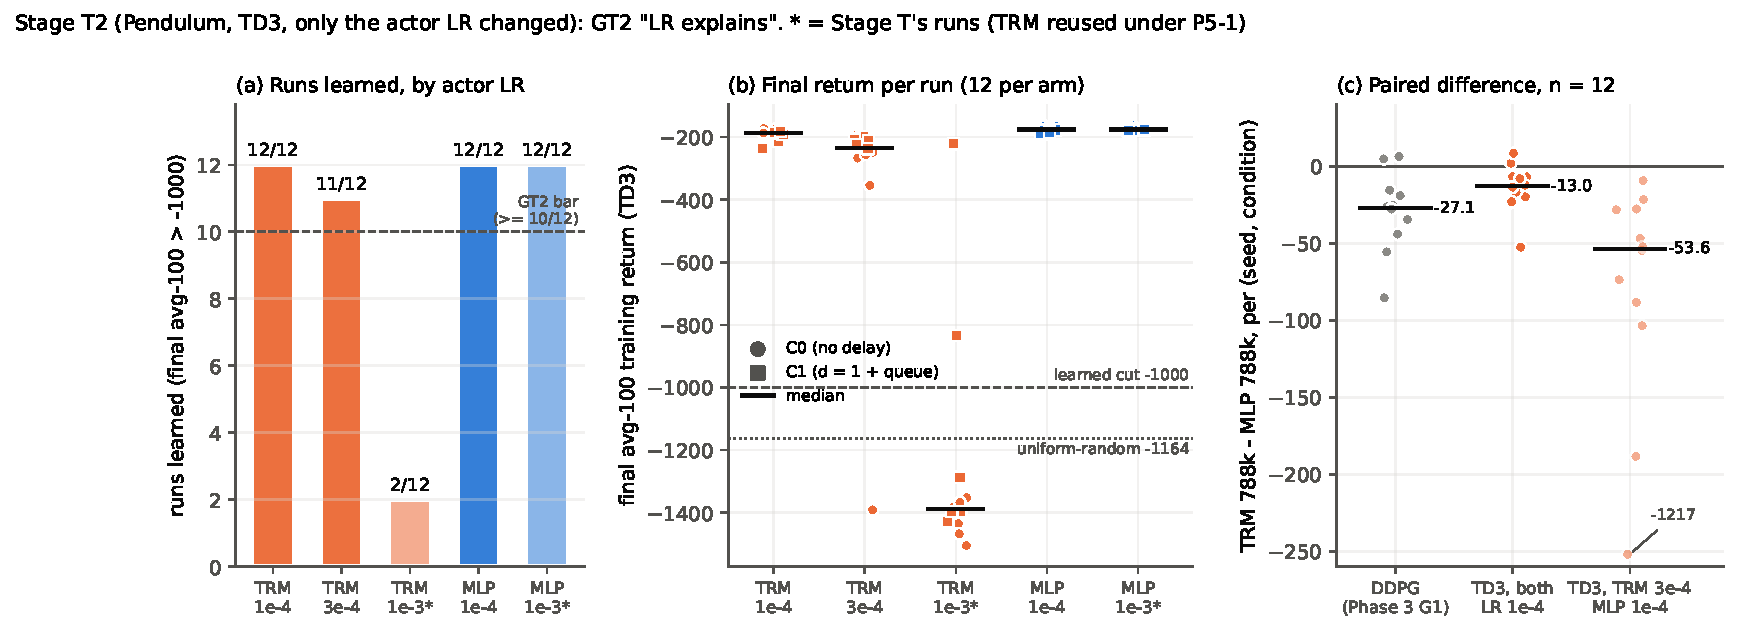
\includegraphics[width=\linewidth,height=0.42\textheight,keepaspectratio]{figures/p5_f1_t2_learned_finals.pdf}
\caption{Stage T2: runs learned and final return by actor LR, and the paired difference against Phase 3's DDPG contrast}
\end{figure}



\subsection*{4.3 Secondary and exploratory measures}\addcontentsline{toc}{subsection}{4.3 Secondary and exploratory measures}



\begin{center}\small\begin{tabular}{>{\raggedright\arraybackslash}p{0.274\linewidth}>{\raggedleft\arraybackslash}p{0.111\linewidth}>{\raggedleft\arraybackslash}p{0.111\linewidth}>{\raggedleft\arraybackslash}p{0.111\linewidth}>{\raggedleft\arraybackslash}p{0.111\linewidth}>{\raggedleft\arraybackslash}p{0.103\linewidth}}
\toprule
Quantity & TRM 1e-4 & TRM 3e-4 & TRM 1e-3 (T) & MLP 1e-4 & MLP 1e-3 (T) \\
\midrule
Critic loss, episodes 51--75 & 59.2 & 68.5 & 118.6 & 44.0 & 41.2 \\
Critic loss, last quarter & 36.0 & 47.4 & 560.9 & 25.4 & 23.7 \\
Runs where late > early & 0/12 & 2/12 & 11/12 & 0/12 & 0/12 \\
Median wall-clock on L40S (runs) & 22.69 min (9) & 23.60 min (6) & 23.37 min (1) & 2.04 min (12) & 2.14 min (3) \\
\bottomrule
\end{tabular}\end{center}



\begin{center}\small\begin{tabular}{>{\raggedright\arraybackslash}p{0.483\linewidth}>{\raggedleft\arraybackslash}p{0.069\linewidth}>{\raggedleft\arraybackslash}p{0.189\linewidth}>{\raggedleft\arraybackslash}p{0.137\linewidth}}
\toprule
Paired (n = 12), exploratory & Median & Positive / above 1 & p (two-sided) \\
\midrule
Late critic loss ratio, TRM @ 1e-4 / MLP @ 1e-4 & 1.50$\times$ & 12/12 & --- \\
Late critic loss ratio, TRM @ 3e-4 / MLP @ 1e-4 & 1.75$\times$ & 12/12 & --- \\
Eval last-5, TRM @ 1e-4 $-$ MLP @ 1e-4 & $-$6.68 & 2/12 & 0.039 \\
Eval last-5, TRM @ 3e-4 $-$ MLP @ 1e-4 & $-$19.06 & 2/12 & 0.039 \\
Final, MLP @ 1e-4 $-$ MLP @ 1e-3 (Stage T) & $-$0.03 & 6/12 & 1.00 \\
Final, TRM @ 1e-4 $-$ TRM @ 3e-4 & +37.89 & 10/12 & 0.039 \\
\bottomrule
\end{tabular}\end{center}



\emph{Source: \texttt{figures/\allowbreak{}derived\_\allowbreak{}numbers\_\allowbreak{}p5.\allowbreak{}json} (\texttt{t2.per\_arm}, \texttt{t2.pairs}).}



\begin{figure}[htbp]\centering
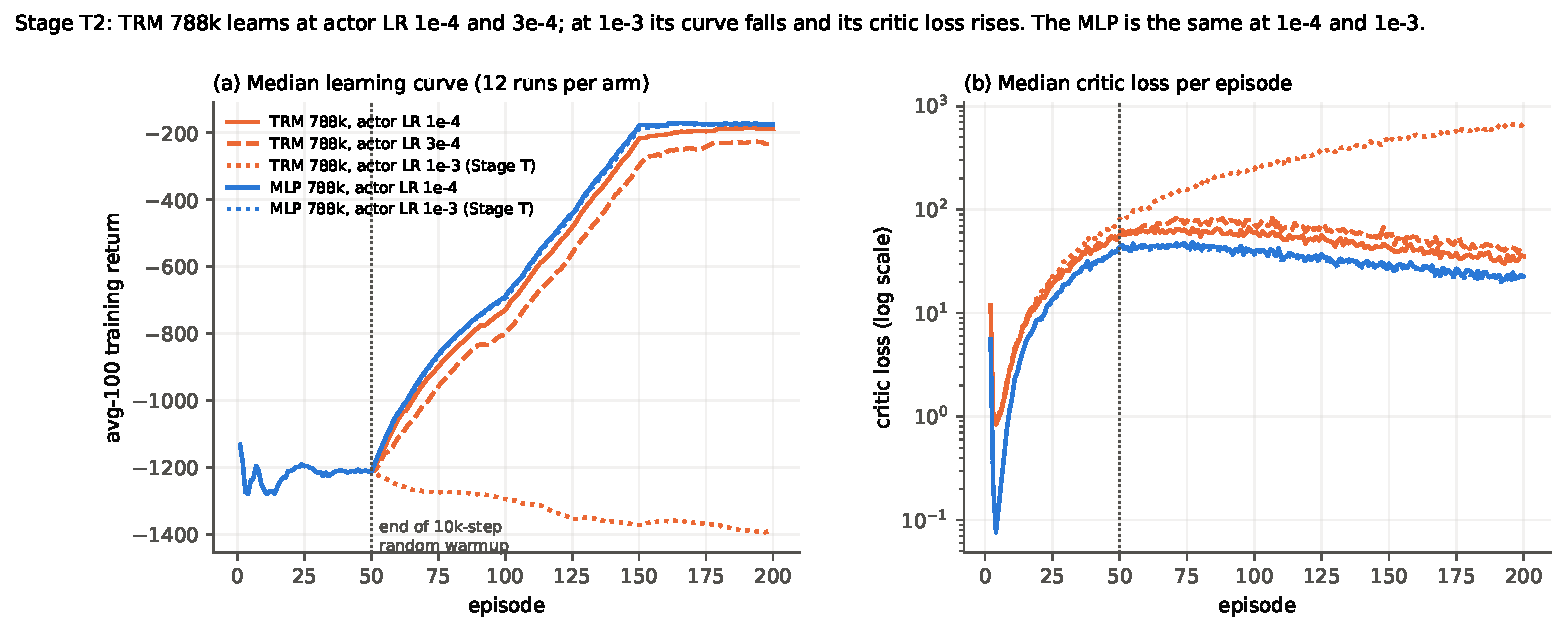
\includegraphics[width=\linewidth,height=0.42\textheight,keepaspectratio]{figures/p5_f2_t2_curves.pdf}
\caption{Stage T2: median learning curves and critic loss per episode}
\end{figure}



\section*{5. Discussion}\addcontentsline{toc}{section}{5. Discussion}



\textbf{What the numbers show.} Lowering only the actor learning rate turns TD3 from a setting in which TRM 788k mostly fails into one in which it learns every run. Its median learning curve rises after the 50-episode warmup, tracking a little below the MLP's, where at 1e-3 it fell. Its critic loss falls through training in every run, from 59.2 to 36.0, where at 1e-3 it rose in 11 of 12. The MLP is indifferent to the same tenfold change: medians $-$176.14 and $-$175.92, paired difference $-$0.03 (6/12), and the same critic loss. Once TRM trains, it still trails the parameter-matched MLP: by a median 12.98 in training return (10/12 pairs negative), by 6.68 on the greedy policy (10/12), with a late critic loss 1.50$\times$ the MLP's in every pair.



\textbf{How robust.} The learned counts leave little room for doubt: 12/12 against 2/12 at the same seeds and conditions, with every 1e-4 run ending between $-$171.7 and $-$237.4. The primary contrast is weaker: 2/12 positive is exactly the pre-registered n = 12 threshold's p (0.039), and the two positive pairs are small (+2.01, +8.38). The direction matches every earlier matched-capacity TRM-versus-MLP contrast in the project. The pooled seed SD (14.50) is about the size of the median deficit, so the deficit is consistent rather than large.



\textbf{Competing explanations for the Stage T failure, revisited.} Stage T listed five, none tested (\texttt{phase4/\allowbreak{}report/\allowbreak{}stage\_\allowbreak{}T.\allowbreak{}md} \S{}4).



\begin{center}\small\begin{tabular}{>{\raggedright\arraybackslash}p{0.264\linewidth}>{\raggedright\arraybackslash}p{0.670\linewidth}}
\toprule
Explanation & After Phase 5 \\
\midrule
Actor LR 1e-3 too high for TRM & \textbf{Supported by the pre-registered test.} Lowering it alone restores learning (12/12 at 1e-4) \\
Other TD3 settings (batch 256, twin critics, target smoothing, policy delay) & \textbf{Not sufficient on their own.} All were unchanged at 1e-4, and TRM trained \\
Width-dependent instability & Not tested here (only TRM 788k ran). If width matters, it does so through the step size: the same width trains at 1e-4 \\
Critic divergence drives the failure & \textbf{Downstream of the actor step size.} The critic LR (1e-3) was the same in every arm, and the critic diverged only at the high actor rate. The data do not separate "the actor's large steps destabilise the critic's targets" from "a policy stuck near random inflates the TD error" \\
Too few learning episodes & \textbf{Excluded.} The same 200-episode budget and 50-episode warmup suffice at 1e-4 \\
\bottomrule
\end{tabular}\end{center}



\textbf{How it compares with Phase 3 under DDPG} (cross-stage, descriptive). At 1e-4 under TD3, TRM 788k $-$ MLP 788k is $-$12.98 (2/12); under DDPG in Phase 3 it was $-$27.14 (2/12). The direction and the count are the same; the median under TD3 is about half the DDPG one, with almost the same pooled seed SD (14.50 against 14.71). The value-fit ratio is 1.50$\times$ under TD3 at 1e-4 against 1.89$\times$ under DDPG. The absolute medians are close too: TRM $-$187.69 under TD3 against $-$207.95 under DDPG, MLP $-$176.14 against $-$177.32. TD3 at a matched actor rate thus reproduces Phase 3's qualitative picture: a modest, consistent TRM deficit with a worse value fit.



\textbf{A new observation: TRM is much more sensitive to the actor learning rate} (exploratory). The MLP's results are unchanged by a tenfold change in actor rate. TRM's go from 12/12 learned to 2/12. Even the threefold step from 1e-4 to 3e-4 costs TRM a median 37.89 (10/12 pairs) and one collapsed run. This matches Phase 4's Stage C under DDPG, where all three $\times$3-actor-LR cells fell below the default in 3/3 seeds with the grid's highest critic losses. Across two algorithms, then, the recursive trunk tolerates a large actor step poorly. That fits the reading the project has given since Phase 3: the weight-tied, normalised recursive cell behaves like a feed-forward block that is harder to optimise. It does not identify a mechanism. Large actor updates through 21 applications of one shared cell could plausibly produce larger changes in the action map per step than the same update through an MLP, but nothing here measures that.



\textbf{What it constrains.} The alternative reading of Stage T, that TRM is simply incompatible with TD3, is excluded; so is the reading of GT's pass as evidence of a large architectural deficit. What remains is the Phase 3 result, now under a second algorithm.



\textbf{What it does not show.} The size of TRM's deficit at its best TD3 setting, since lower rates were not tried; whether a different MLP rate would change the contrast (the MLP's insensitivity between 1e-4 and 1e-3 suggests not, across stages); any result beyond Pendulum-v1; and the mechanism of TRM's LR sensitivity.



\section*{6. Deviations from the plan}\addcontentsline{toc}{section}{6. Deviations from the plan}



\begin{itemize}
\item \textbf{Amendment P5-1} (2026-10-10, before data): the 1e-3 arm reuses Stage T's runs; 36 jobs instead of 48. Recorded in \texttt{gates.json} with its caveat.
\item \textbf{No other deviations.} All 36 jobs completed on the first submission; the gate was evaluated once, from complete data.
\end{itemize}



\section*{7. Threats to validity}\addcontentsline{toc}{section}{7. Threats to validity}



\begin{enumerate}
\item \textbf{The threshold} ($-$1000) separates "learned" from "near random", not good from mediocre. It does not decide the result: across all five arms the lowest learned final is $-$834.3 (TRM at 1e-3, C1 seed 5) and the highest unlearned final is $-$1287.1 (TRM at 1e-3, C1 seed 1), so any cut between them gives the same counts.
\item \textbf{Three LR points.} The pass shows the failure is LR-sensitive, not that 1e-4 is TRM's best TD3 actor rate.
\item \textbf{MLP control at one new LR.} The 3e-4 contrast mixes architecture with LR and is reported as such.
\item \textbf{Hardware.} Runs are not bit-reproducible across GPU models (Phase 4 B0). All new MLP runs ran on L40S; new TRM runs on four GPU models; the reused arm mostly on V100 and A100. Hardware variation is part of the seed variation, and it is not balanced across arms.
\item \textbf{Reuse of Stage T.} Same configuration, byte-identical code, but a different batch of jobs submitted three days earlier.
\item \textbf{One environment, one algorithm configuration otherwise unchanged.} Every decisive result in the project remains on Pendulum-v1.
\item \textbf{Exploratory numbers.} The critic-loss windows and ratios, the eval contrasts, the MLP-vs-MLP and TRM-vs-TRM comparisons and the wall-clock figures were computed while writing and are labelled exploratory.
\end{enumerate}



\section*{8. What Phase 5 changes about the Phase 0--4 conclusions}\addcontentsline{toc}{section}{8. What Phase 5 changes about the Phase 0--4 conclusions}



\begin{center}\small\begin{tabular}{>{\raggedright\arraybackslash}p{0.380\linewidth}>{\raggedright\arraybackslash}p{0.554\linewidth}}
\toprule
Phase 0--4 conclusion & After Phase 5 \\
\midrule
G1 holds under TD3 in sign, but by optimisation failure; the magnitude was not measured (GT caveat) & \textbf{Resolved.} At a matched actor LR of 1e-4, TRM 788k $-$ MLP 788k is $-$12.98 (2/12, p = 0.039): the same direction and count as DDPG's $-$27.1 (2/12), with a smaller median \\
TRM is fragile under TD3 (cause untested) & \textbf{Cause identified:} the actor learning rate. At 1e-4 TRM learns 12/12, at 3e-4 11/12, at 1e-3 2/12 \\
TRM fits its value function worse (1.45$\times$, 1.89$\times$ under DDPG; 3.83$\times$, 24.91$\times$ under \texttt{td3.yaml}) & \textbf{Holds under TD3 at a matched LR:} 1.50$\times$ at 1e-4 (12/12). The 24.91$\times$ was mostly the divergence \\
Untuned learning rates ruled out within $\times$0.3--$\times$3 (DDPG, Stage C) & \textbf{Extended in kind:} under TD3 the default actor rate was wrong for TRM, but at a better rate TRM still trails; raising TRM's actor rate hurts under both algorithms \\
One learning algorithm (threat) & \textbf{Addressed for the capacity contrast at Pendulum scale:} the attribution holds under DDPG and TD3 at matched, sensible LRs \\
Complexity scaling (H1) untested & \textbf{Unchanged} \\
Use the MLP & \textbf{Unchanged.} If a recursive trunk is used under TD3, use the DDPG-like actor rate (1e-4); TRM 788k still costs about 11$\times$ the MLP's training time on the same GPU model \\
\bottomrule
\end{tabular}\end{center}



\section*{9. Reproducibility}\addcontentsline{toc}{section}{9. Reproducibility}



\begin{itemize}
\item \textbf{Plan and rules:} \texttt{phase5/\allowbreak{}plan/\allowbreak{}plan.\allowbreak{}md}; \texttt{experiments/\allowbreak{}phase5/\allowbreak{}gates.\allowbreak{}json}.
\item \textbf{Job tooling:} \texttt{experiments/\allowbreak{}phase5/\allowbreak{}p5.\allowbreak{}py} (stage \texttt{t2}), \texttt{sync.sh}, \texttt{poll.sh}; frozen snapshot \texttt{p5code/t2} on Katana.
\item \textbf{Analysis:} \texttt{experiments/\allowbreak{}phase5/\allowbreak{}gates\_\allowbreak{}eval.\allowbreak{}py gt2} $\rightarrow$ \texttt{experiments/\allowbreak{}analysis\_\allowbreak{}p5\_\allowbreak{}t2.\allowbreak{}json} (reads \texttt{phase5/\allowbreak{}results/\allowbreak{}results\_\allowbreak{}p5t2/\allowbreak{}} and, for the reused arms, \texttt{phase4/\allowbreak{}results/\allowbreak{}results\_\allowbreak{}p4t/\allowbreak{}}).
\item \textbf{Figures and exploratory numbers:} \texttt{experiments/\allowbreak{}phase5/\allowbreak{}make\_\allowbreak{}figures\_\allowbreak{}phase5.\allowbreak{}py} $\rightarrow$ \texttt{phase5/\allowbreak{}report/\allowbreak{}figures/\allowbreak{}} (\texttt{p5\_\allowbreak{}f1\_\allowbreak{}t2\_\allowbreak{}learned\_\allowbreak{}finals}, \texttt{p5\_\allowbreak{}f2\_\allowbreak{}t2\_\allowbreak{}curves}, \texttt{p5\_\allowbreak{}f3\_\allowbreak{}project\_\allowbreak{}map}, \texttt{derived\_\allowbreak{}numbers\_\allowbreak{}p5.\allowbreak{}json}).
\item \textbf{Documents:} \texttt{phase5/\allowbreak{}report/\allowbreak{}build.\allowbreak{}py <file>.\allowbreak{}md} (Markdown $\rightarrow$ LaTeX $\rightarrow$ PDF with tectonic).
\item \textbf{One training run,} e.g. TRM 788k at actor LR 1e-4, C1, seed 1 (core overrides; \texttt{p5.py} adds logging and output-folder fields):
\end{itemize}



{\small\begin{verbatim}
python3 -u main.py arch=td3 model=trm env=pendulum delay=fixed delay.value=1 \
  augment_obs=true arch.total_episodes=200 seed=1 \
  wandb.enabled=false eval_every=10 run_tag=alr1e-4 arch.actor_lr=1e-4
\end{verbatim}}



\section*{Appendix A --- Gate outcome as recorded}\addcontentsline{toc}{section}{Appendix A --- Gate outcome as recorded}



\begin{center}\small\begin{tabular}{>{\raggedright\arraybackslash}p{0.079\linewidth}>{\raggedright\arraybackslash}p{0.115\linewidth}>{\raggedright\arraybackslash}p{0.712\linewidth}}
\toprule
Gate & Status & Detail (from \texttt{experiments/\allowbreak{}phase5/\allowbreak{}gates.\allowbreak{}json}) \\
\midrule
GT2 & LR explains & trm 1e-4: 12/12 learned (median $-$187.69); trm 3e-4: 11/12 learned (median $-$234.56); trm 1e-3: 2/12 learned (median $-$1389.27); dnn\_large 1e-4: 12/12 learned (median $-$176.14); dnn\_large 1e-3 (Stage T): 12/12 learned (median $-$175.92). trm@1e-4 $-$ dnn\_large@1e-4: median $-$12.98, 2/12 positive, two-sided p = 0.0386 [LR-matched (primary)]; trm@3e-4 $-$ dnn\_large@1e-4: median $-$53.6, 0/12 positive, two-sided p = 0.0005 [unequal actor LRs (TRM 3e-4 vs MLP 1e-4)]. \\
GT (Phase 4) & pass (unchanged) & Its caveat's "likely contributor, untested" is now tested by GT2. Phase 4's \texttt{gates.json} is not edited. \\
\bottomrule
\end{tabular}\end{center}



\emph{The GT2 detail is quoted from \texttt{gates.json}, with the arm separator "|" written as a space.}



\subsection*{References}\addcontentsline{toc}{subsection}{References}



Fujimoto, S., van Hoof, H. \& Meger, D. (2018). \emph{Addressing Function Approximation Error in Actor-Critic Methods.} ICML $\cdot$ Jolicoeur-Martineau, A. (2025). \emph{Less is More: Recursive Reasoning with Tiny Networks.} arXiv:2510.04871 $\cdot$ Lillicrap, T. P. et al. (2016). \emph{Continuous control with deep reinforcement learning.} ICLR $\cdot$ Towers, M. et al. (2024). \emph{Gymnasium.} arXiv:2407.17032
\end{document}
